\documentclass[a4paper,12pt]{article}

\usepackage{a4wide}
\usepackage{amsfonts}
\usepackage{amsmath}
\usepackage{amssymb}
\usepackage{lipsum}

\usepackage{graphicx}  % For including images

\usepackage{xcolor}  % For a colorfull presentation
\usepackage{listings}  % For presenting code 

\usepackage{hyperref}

% Definition of a style for code, matter of taste
\lstdefinestyle{mystyle}{
  language=Python,
  basicstyle=\ttfamily\footnotesize,
  backgroundcolor=\color[HTML]{F7F7F7},
  rulecolor=\color[HTML]{EEEEEE},
  identifierstyle=\color[HTML]{24292E},
  emphstyle=\color[HTML]{005CC5},
  keywordstyle=\color[HTML]{D73A49},
  commentstyle=\color[HTML]{6A737D},
  stringstyle=\color[HTML]{032F62},
  emph={@property,self,range,True,False},
  morekeywords={super,with,as,lambda},
  literate=%
    {+}{{{\color[HTML]{D73A49}+}}}1
    {-}{{{\color[HTML]{D73A49}-}}}1
    {*}{{{\color[HTML]{D73A49}*}}}1
    {/}{{{\color[HTML]{D73A49}/}}}1
    {=}{{{\color[HTML]{D73A49}=}}}1
    {/=}{{{\color[HTML]{D73A49}=}}}1,
  breakatwhitespace=false,
  breaklines=true,
  captionpos=b,
  keepspaces=true,
  numbers=none,
  showspaces=false,
  showstringspaces=false,
  showtabs=false,
  tabsize=4,
  frame=single,
}
\lstset{style=mystyle}

\begin{document}
\title{Machine Learning A (2024)\\Home Assignment 2}
\author{Carlo Rosso rkm957}
\date{}
\maketitle

% Please leave the table of contents as is, for the ease of navigation for TAs
\tableofcontents % Generates the table of contents
\newpage % Start a new page after the table of contents


\section{Linear Regression (50 points)}

\textbf{Taks 1}
\begin{lstlisting}
class LinearRegression:
    w = np.random.normal(loc=0, scale=0.3, size=2)
        
    def predict(self, x) -> float:
        x = np.append(x, 1)
        return self.w.T @ x
        
    def loss(self, xs, ys) -> float:
        error = [(t - self.predict(x))**2 for t, x in zip(ys, xs)]
        return np.sum(error) / len(ys)
        
    def train(self, xs, ys):
        x = np.array([np.append(x, 1) for x in xs])
        self.w = np.linalg.inv(x.T @ x) @ x.T @ ys
\end{lstlisting}

\vspace{1em}
\noindent\textbf{Task 2}\\
The parameters of the model are the weights $a = 0.259$ and\\
$b = 0.0315$; while the mean-squared-error is
$\mathcal{L} = 34.8$.

I obtained the parameters and the result of the loss function by training the
following model:

\begin{lstlisting}
class NonLinearModel(LinearRegression):
    def predict(self, x) -> float:
        return math.exp(super().predict(x))
    
    def train(self, xs, ys):
        super().train(xs, np.log(ys))
\end{lstlisting}

\vspace{1em}
\noindent\textbf{Task 3}\\
I am not sure how to answer to this question: I tried to derivate the loss of
the first model and I obtained the following result:

\begin{equation}
	\sum_{i=1}^{n} e^{2w^Tx_i} \cdot x_i - \sum_{i=1}^{n} 2y_i \cdot e^{w^t x_i} = 0
\end{equation}
where $w^Tx_i = a \cdot \bar{x}_i + b$. At this point I do not know how to keep
going. So I am not able to compute the best parameters for the model in the left
side of the inequality. While the a and b for the model described in the right
side of the inequality are reported in the previous answer.

\vspace{1em}
\noindent\textbf{Task 4}\\
\begin{figure}[htbp]
	\centering
	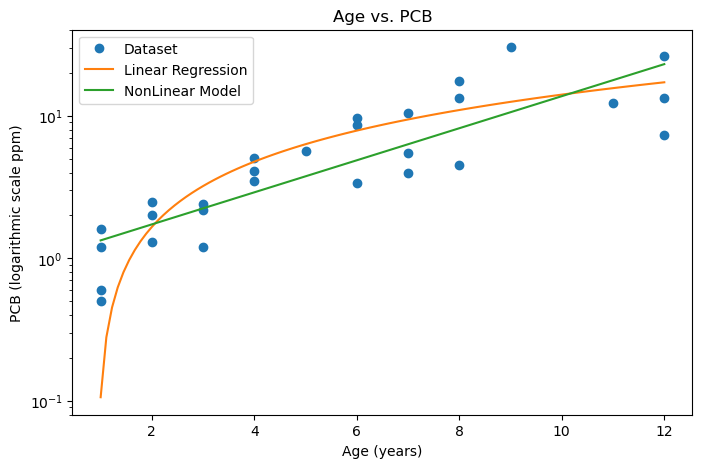
\includegraphics[width=0.5\textwidth]{a2-t4}
	\caption{Non-linear model's predictions compared to the true values.}
\end{figure}

\vspace{1em}
\noindent\textbf{Task 5}\\
$R^2 = 0.357$. Follows the definition of the function through which I compute
$R^2$:

\begin{lstlisting}
def r_squared(y_true, y_pred):
    num = np.sum([(y - p)**2 for p, y in zip(y_pred, y_true)])
    den = np.sum([(y - np.mean(y_true))**2 for y in y_true])
    return 1 - (num / den)
\end{lstlisting}

I will discuss the possible values of $R^2$:
\begin{itemize}
	\item $R^2 = 1$: the model perfectly fits the data, indeed
	      \begin{equation}
		      n \cdot \mathcal{L} = \sum_{i=1}^{n} (y_i - h(x_i))^2 = 0.
	      \end{equation}

	\item $R^2 = 0$: the model is predicting the mean of the target values,
	      indeed
	      \begin{equation}
		      \sum_{i=1}^{n} (y_i - h(x_i))^2 = \sum_{i=1}^{n} (y_i - \bar{y})^2.
	      \end{equation}

	\item $R^2 < 0$: the model is worse than just predicting the mean of the
	      target values, indeed
	      \begin{equation}
		      \sum_{i=1}^{n} (y_i - h(x_i))^2 > \sum_{i=1}^{n} (y_i - \bar{y})^2.
	      \end{equation}
\end{itemize}

\vspace{1em}
\noindent\textbf{Task 6}\\
$\mathcal{L} = 28.1$. Follows the code to implement the model:

\begin{lstlisting}
class NonLinearModel2(NonLinearModel):
    def predict(self, x) -> float:
        return super().predict(np.sqrt(x))
    
    def train(self, xs, ys):
        super().train(np.sqrt(xs), ys)
\end{lstlisting}

\begin{figure}[htbp]
	\centering
	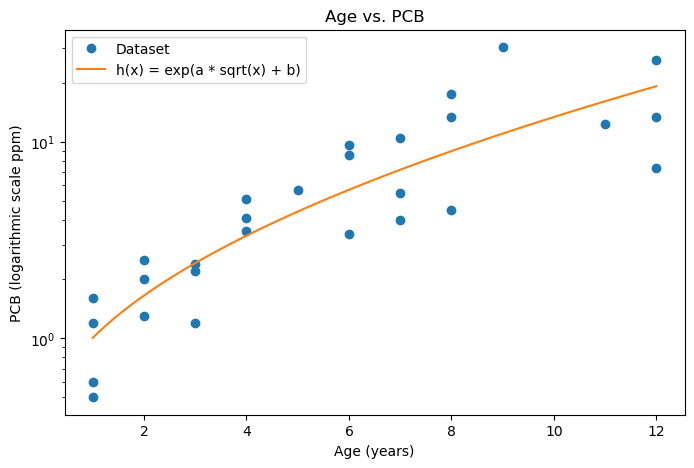
\includegraphics[width=0.5\textwidth]{a2-t6}
	\caption{$h(x) = exp(a \sqrt(x) + b)$ model's predictions compared to the true values.}
\end{figure}

$R^2 = 0.482$. We have three values for the two models we can
compare and all three show that the latest model is better than the previous
one:
\begin{itemize}
	\item loss: $28.1< 34.8$, which means that the
	      mean-squared-error is lower for the latest model, which means that the
	      model better fit the data;

	\item plot of the predictions: we can see also by the plot of the
	      predictions that the latest model's predictions fits better the true
	      values;

	\item $R^2$: finally, we can compare $R^2$. Actually the only thing that
	      changes in the $R^2$ formula is the numerator $\sum_{i=1}^{n} (y_i -
		      h(x_i))^2$, which is $n \cdot \mathcal{L}$, so technically we
	      already discussed this point. Anyway, also $R^2$ shows that the
	      latest model is better, indeed $0.482 > 0.357$ and its $R^2$ value is
	      closer to 1.
\end{itemize}


\section{The Role of Independence (13 points)}

Considering the definition of expeted value:

\begin{equation}
	\mathbb{E}[X] = \sum_{x \in \{0, 1\}} x \cdot P(X = x) = \mu
\end{equation}

and the definition of mean:
\begin{equation}
	\bar{X} = \frac{1}{n} \sum_{i=1}^{n} X_i
\end{equation}

We are asked to design identically distributed random variables $X_1, \dots,
	X_n$ such that $|\mu - \bar{X}| \geq 0.5$. We can design the following
distribution:

\begin{equation}
	X_i = \begin{cases}
		1 & \text{with probability } 0.5 \\
		0 & \text{with probability } 0.5
	\end{cases}
\end{equation}

In this case, $\mathbb{E}[X] = 1 \cdot 0.5 + 0 \cdot 0.5 = 0.5$. So we decide
the correlation between the random variables $X_i$ to be equal to 1. Here
follows the definition of the correlation:
\begin{equation}
	\text{Corr}_{x,y} = \frac{\sum_{i=1}^n (x_i - \bar{x})(y_i - \bar{y})}
	{\sqrt{\sum_{i=1}^n (x_i - \bar{x})^2 \sum_{i=1}^n (y_i - \bar{y})^2}} = 1
\end{equation}

for every $x, y \in \{X_1, \dots, X_n\}$.
It basically means that $X_i = X_j$ for every $i, j$ in $\{1, \dots, n\}$.
Therefore, the random variables $X_i$ are not independent and particularly, if
$X_1 = 1$, then $X_2 = 1$, $X_3 = 1$, and so on. In this case, the mean of the
random variables is equal to 1, while the expected value is equal to 0.5. So
the difference between the mean and the expected value is equal to 0.5.
Therefore the disequality $|\mu - \bar{X}| \geq 0.5$ holds.
On the other hand if we consider $X_1 = 0$, then $X_2 = 0$, $X_3 = 0$, and so
on. In this case, the mean of the random variables is equal to 0, while the
expected value is equal to 0.5. So the difference between the mean and the
expected value is equal to 0.5. Therefore the disequality $|\mu - \bar{X}| \geq
	0.5$ holds, with probability 1.

\section{Confidence Intervals for Bernoulli (17 points)}

\vspace{1em}
\noindent\textbf{Task 1}\\
The 0.95-CI for $\mu$ using Hoedffding's inequality is $[0.703, 0.876]$.
I computed the CI using the following function:

\begin{lstlisting}
def hoeffding_ci(n, mean, delta):
    delta = 1 - delta
    margin = math.sqrt(1 / 2 / n * math.log(2 / delta))
    return max(mean - margin, 0), min(mean + margin, 1)
\end{lstlisting}

Then I importend the dataset \texttt{S.csv} and I computed the mean $\mu$ on the
dataset and I used the $len(S)$ as the number of samples $n$. The \texttt{delta}
is given by the question and it is equal to $0.95$.

\vspace{1em}
\noindent\textbf{Task 2}\\
Just as before I used \texttt{delta} equal to $0.98$ and I computed the 0.98-CI:
$[0.693, 0.886]$.

\vspace{1em}
\noindent\textbf{Task 3}\\
Since 0.95 and 0.98 aren't far from each other the two intervals we obtained
are very similar, indeed their margin from the mean differ of
$0.010$.

\section{Comparison of Markov's, Chebyshev's, and Hoeffding's Inequalities (20 points)}

Follows the information about the distribution we are considering:

\begin{align}
	x_i             & = \begin{cases}
		                    1 & \text{with probability } 1/6 \\
		                    0 & \text{with probability } 5/6
	                    \end{cases}
	\\
	\mathbb{E}[x_i] & = 1 \cdot 1/6 + 0 \cdot 5/6 = 1/6          \\
	X               & = \sum_{i=1}^{n} x_i                       \\
	X               & \in \{0, \dots, n\}                        \\
	\mathbb{E}[X]   & = \sum_i^{n} \mathbb{E}[x_i] = \frac{n}{6} \\
\end{align}

We are asked to derive uppoer bounds for the following probability:

\begin{equation}
	p = \mathcal{P}(X \geq n/4)
\end{equation}

with Markov's, Chebyshev's, and Hoeffding's inequalities.

\vspace{1em}
\noindent\textbf{Task 1 - Markov's inequality}\\

Markov's inequality is defined as follow:

\begin{equation}
	\mathbb{P}(X \geq a) \leq \frac{\mathbb{E}[X]}{a}
\end{equation}

and we have all the information to compute the upper bound for $p$:

\begin{equation}
	p = \mathbb{P}(X \geq n/4) \leq \frac{n/6}{n/4} = \frac{n}{6} \cdot \frac{4}{n} = \frac{2}{3}
\end{equation}

\vspace{1em}
\noindent\textbf{Task 2 - Chebyshev's inequality}\\

Chebyshev's inequality is defined as follow:

\begin{equation}
	\mathbb{P}(|X - \mathbb{E}[X]| \geq a) \leq \frac{\text{Var}[X]}{na^2}
\end{equation}

First of all we need to change the formulation because we want to have $X \geq
	n/4$ and not $|X - \mathbb{E}[X]| \geq a$. We can write the value of
$\mathbb{E}[X]$ and we get $|X - n/6| \geq n/4$. Now we have two cases:
\begin{equation}
	\begin{cases}
		X - n/6 \geq n/4 \\
		X - n/6 \leq -n/4
	\end{cases}
\end{equation}

But we are actaully interested only in the first case. So we can rewrite:

\begin{align}
	\mathbb{P}(X - n/6 \geq a)                                = \mathbb{P}(X - n/6 \leq -a) \\
	\mathbb{P}(X - n/6 \geq a) + \mathbb{P}(X - n/6 \leq -a) \leq \frac{\text{Var}[X]}{na^2}
\end{align}

So we get:
\begin{align}
	 & \mathbb{P}(X - n/6 \geq a) + \mathbb{P}(X - n/6 \leq -a) \leq \frac{\text{Var}[X]}{na^2}                   \\
	 & 2 \cdot \mathbb{P}(X - n/6 \geq a)                       \leq \frac{\text{Var}[X]}{na^2}                   \\
	 & \mathbb{P}(X - n/6 \geq a)                               \leq \frac{1}{2} \cdot \frac{\text{Var}[X]}{na^2} \\
	 & \mathbb{P}(X \geq a + n/6)                               \leq \frac{1}{2} \cdot \frac{\text{Var}[X]}{na^2} \\
\end{align}

Now we impose $a + n/6 = n/4$ and we get $a = n / 12$. So we get the upper bound
for $p$:

\begin{align}
	p = \mathbb{P}(X \geq n/4) \leq \frac{1}{2} \cdot \frac{\text{Var}[X]}{n(n/12)^2} \\
	p = \mathbb{P}(X \geq n/4) \leq \frac{12 ^ 2}{2} \cdot \frac{\text{Var}[X]}{n^3}
\end{align}

\vspace{1em}
\noindent\textbf{Task 3 - Hoeffding's inequality}\\

Hoeffding's inequality is defined as follow:

\begin{equation}
	\mathbb{P}(X - \mathbb{E}[X] \geq a) \leq e^{-2a^2/n}
\end{equation}

So it is straightforward to compute the upper bound for $p$: we need only to
compute $a$.

\begin{align}
	X - \mathbb{E}[X] & \geq a       \\
	X - n/6           & \geq a       \\
	X                 & \geq a + n/6
\end{align}

And we want to have $a + n/6 = n/4$, so $a = n/12$. So we get the upper bound:

\begin{equation}
	p = \mathbb{P}(X \geq n/4) \leq e^{-2(n/12)^2/n} = e^{-2n/12^2}
\end{equation}

\end{document}
